\section[陀螺]{陀\qquad 螺}\label{sec:10.05}

陀螺是一个典型的刚体运动问题。

所谓陀螺是一个绕轴快速自转的物体,如图\ref{fig:10.21} 所示。它的
\begin{wrapfigure}[12]{l}{13em}
    \centering
    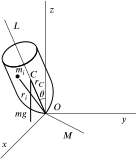
\includegraphics{figure/fig10.21}
    \caption{陀螺}
    \label{fig:10.21}
\end{wrapfigure}
转轴不是固定的,但其顶点是固
定的,如固定于原点$ O $处。根据
经验,我们知道,这样一个快速
自旋的陀螺的轴总是围绕竖直轴
转动,并扫出一个圆锥面。现在
我们根据经典力学原理来研究一
下这种运动情况。特别是想计算
出自旋轴绕竖直轴转动的角速
度。

由于现在并不是绕固定轴
的转动,我们应当用转动方程
\eqref{eqn:10.04.04}作为研究的起点,即

% 307.jpg
\clearpage~\vspace{-1.56em}
\begin{equation}\label{eqn:10.05.01}
    \frac {  \dif \vec{L} } {  \dif t } = \vec{M}
\end{equation}
在每一瞬时,陀螺绕其自旋轴转动,其角速度为$ \vec{\omega} $,称为自旋角
速度。一般地说,陀螺的总角动量$\vec{L}$与$\vec{\omega}$方向并不相同。但若陀螺
的形状是对称的且外力矩$\vec{M}$较小,则可以近似地认为$\vec{L}$与$\vec{\omega}$同方
向。对于我们现在的情况,只有重力相对于$ O $点有力矩。由于维
持陀螺固定在$ O $点,当然也有力在$ O $点作用于陀螺,但这种力对$ O $
点的力矩显然为零。取一质量元$ m _ i $,其重力矩为$  \vec{r} _ { i } \times m _ { i } \vec{g}   $,故总
的重力矩为
\begin{equation*}
    \begin{split}
        \vec{M} &= \sum_{ i = 1 } ^ n \left( \vec{r} _ i \times m _ { i } \vec{g} \right) \\
                &= \Bigg( \sum_{ i = 1 } ^ n m _ i \vec{r} _ { i } \Bigg) \times \vec{g} \\
                &= \Bigg( \frac { \sum _{ i = 1 } ^ n m _ i \vec{r} _ i } { m } \Bigg) \times m \vec{g} \\
                &= \vec{r} _ { c } \times m \vec{g}
    \end{split}
\end{equation*}
\begin{wrapfigure}[12]{r}{13em}
    \vspace{-1em}
    \centering
    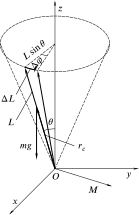
\includegraphics{figure/fig10.22}
    \caption{陀螺的动力学}
    \label{fig:10.22}
\end{wrapfigure}
式中$ \vec{r} _ c $是陀螺质心的位置矢量。
对于我们现在讨论的对称陀螺的
情况,$ \vec{r} _ c $沿自旋轴,故与$ \vec{L} $平行
或反平行。

如果快速转动的陀螺放得很
正,自旋轴垂直于水平面,于是
$ \vec{M} = 0 $  ,所以$ \vec{L} = \text{不变量} $,转动轴
不变,始终在竖直的方向。

如果陀螺放得不正,自旋轴
与竖直方向成角(图\ref{fig:10.21}),则
$ \vec{M} = \vec{r} _ { c } \times m \vec{g} \ne 0 $, $ \vec{M} $在垂直于$ \vec{r} _ c $和
$ m\vec{g} $所决定的平面(图\ref{fig:10.22},为清
% 308.jpg
楚起见,图中未画出陀螺本身形状),即$ \vec{M} $垂直于$\vec{L}$。由式\eqref{eqn:10.05.01},
在$ \Delta t $时间里,$\vec{L}$的变化应为
\begin{equation*}
    \Delta \vec{L} = \vec{M} \Delta t
\end{equation*}
故角动量变化量$ \Delta \vec{L} $应象$\vec{M}$一样垂直于$\vec{L}$。在时间间隔$ \Delta t $末,陀
螺的角动量为$ \vec{L} + \Delta \vec{L} $,因为$ \Delta \vec{L} $始终垂直于$\vec{L}$,所以新的角动量与
原来的角动量有相等的数值,但方向不同。又因$ \Delta \vec{L} $始终垂直于
$ Z $轴,因此,角动量$ L $的顶端就只能是绕一水平圆周的运动。这
就证明了陀螺在斜放时,由于重力矩的作用,除自旋外,自旋轴
还绕着竖直轴($ Z $轴)转动。我们把自旋轴绕竖直轴的转动称为进
动。

由图\ref{fig:10.22} 可求得进动角速率$ \omega _ \text{进} $。用该图中的符号,即有
\begin{align*}
    \omega _ \text{进} &= \frac { \Delta \varphi } { \Delta t } \\
    \beforetext{以及}
        \Delta \varphi &= \frac { \Delta L } { L \sin \theta } \\
            &= \frac { M \Delta t } { L \sin \theta } \\
    \beforetext{又因} M &= r _ { c } m g \sin \theta \\
    \beforetext{故}    \Delta \varphi &= \frac { r _ { c } m g \sin \theta \Delta t } { L \sin \theta } \\
            &= \frac { r _ { c } m g \Delta t } { L }
\end{align*}
最终得到
\begin{equation}\label{eqn:10.05.02}
    \begin{split}
        \omega _ \text{进} &= \frac { \Delta \varphi } { \Delta t } \\
                &= \frac { r _ { c } m g } { L }
    \end{split}
\end{equation}
可见,进动角速率进与角动量的大小$ L $成反比。对于同一陀螺
% 309.jpg
来说,自旋角动量愈大,则进动角速率愈小。

\clearpage
地球就是一个陀螺。地球的自转轴相当于陀螺的轴,自转速
率是每24小时一周。当然,地球的自转中并不存在一个固定的顶
点,与前面讨论的情况不完全相同。但若选择地心(大体也就是
地球的质心)作为基点,则平动与转动相互是分离的,平动部分
是地球绕太阳的公转,而转动部分就类似于一个陀螺。

\vspace{1.5em}
\begin{figure}[h]
    \centering
    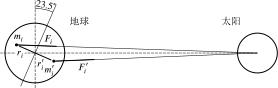
\includegraphics{figure/fig10.23}
    \caption{地球的进动}
    \label{fig:10.23}
\end{figure}

如图\ref{fig:10.23},地球的自转轴并不垂直于地球的公转平面,它与
该平面的法线之间的夹角为$ 23.5 ^ \circ $。如果地球质量分布相对于自
转轴是对称的,则我们可将地球分解为许多相对于该轴对称分布
的质元对,如图\ref{fig:10.23} 中的$ m _ i $与$ m _ i ^ \prime $就是一组对称的质元。太阳作
用在它们上的引力相对于$ O $的力矩为
\begin{equation*}
    \begin{split}
        \vec{M} _ { i } &= r _ { i } \times \vec{F} _ i \\
        \vec{M} _ { i } ^ { \prime } &= r _ { i } ^ { \prime } \times \vec{F} _ i ^ \prime
    \end{split}
\end{equation*}
式中$ \vec{F} _ i,  \vec{F} _ i ^ \prime$分别是太阳对$ m _ i , m _ i ^ \prime $的引力。因为$ \vec{r} _ i = - \vec{r} _i ^ \prime $,所以,
若$ \vec{F} _ i = \vec{F} _ i ^ \prime $,则$\vec{M}$与$\vec{M} ^ \prime$就会方向相反、大小相同,这样它们就相互
抵消。同理,每组质元都有相同的结果,因此,整个地球所受太
阳引力对$ O $点的力矩为零。但是$ \vec{F} _ i $与$ \vec{F} _ i ^ \prime $并不严格相等,因为二者
与太阳的距离并不完全相同。所以,太阳引力相对于$ O $点是有力
矩的,即$\vec{M} ^ \prime$与$\vec{M}$并不严格相抵消。这个力矩使地球自转轴发生进
动。这种现象称为岁差。地球自转轴进动的周期很长,约26,000
年。尽管如此小,在两千年前它就被希腊天文学家发现了。由于
% 310.jpg
这个效应,地球的自转轴实际上并不总是指向北极星。在公元前
2,500年时,“极星”(即自转轴指向的星)是右垣一(即天龙$ \alpha $),
到公元14,000年时,“极星”将是织女星。